\documentclass[a4paper, 11pt, article,oneside,openany]{memoir} %A4 papir, skrift 11, artikel, ensidet print, kapitel kan starte på alle sider

% Sætter horisontal og vertikale margener
\usepackage[paper=a4paper,%
hmargin=1.5in,%
vmargin=0.9in
]{geometry}

% Font encoding og sprog
\usepackage[T1]{fontenc}
\usepackage[utf8]{inputenc}

\usepackage{siunitx}

\sisetup{group-separator = {,}}
\sisetup{per-mode=fraction}

\DeclareSIUnit{\sqrthz}{\ensuremath{\sqrt{\text{\hertz}}}}
\DeclareSIUnit{\voltnoise}{\volt\per\sqrthz}
\DeclareSIUnit{\amperenoise}{\ampere\per\sqrthz}

\usepackage[danish]{babel} % bedre orddeling, minimum to tegn før og efter deling
\usepackage{lmodern}  					% gør  pænere
\usepackage{microtype} 					% laver micro ændringer i text for at udgå luft og orddeling



% Farvepakker
\usepackage[svgnames,dvipsnames,x11names]{xcolor}

% Visning af kildekode
\usepackage{listings}

\lstset{ %
	backgroundcolor=\color{white}, 	% Baggrundsfarve
	basicstyle=\tiny,        			% Tekststørrelse
	breakatwhitespace=true,        		% Kun linjeskift ved mellemrum
	breaklines=true,                 		% Orddeling til
	captionpos=b,                    		% Caption under listing
	commentstyle=\color{mygreen},    	% kommentar farve
	extendedchars=true,              		% lets you use non-ASCII characters; for 8-bits encodings only, does not work with UTF-8
	frame=single,	                   		% Ramme omkring kildekode
	keepspaces=true,                 		% beholder mellemrum (indentation)
	keywordstyle=\color{blue},      	 	% keyword farve
	numbers=left,                    		% Placering af linjenumre (none, left, right)
	numbersep=5pt,                   		% Afstand til linjrenumre
	numberstyle=\tiny\color{mygray}, 	% Linjenummer tekststil
	showspaces=false,                		% show spaces everywhere adding particular underscores; it overrides 'showstringspaces'
	stepnumber=1,                    		% Hver linje har nummer
	tabsize=4,	                   		% Sætter default tabsize til 4 mellemrum
	title=\lstname                   		% filnavn som caption, hvis ikke andet er angivet
}

\usepackage{xcolor}% provides \colorlet
\usepackage{fixme}
\fxsetup{
	status=draft,
	author=,
	layout=inline,
	theme=color
}

\definecolor{fxnote}{rgb}{0.8000,0.0000,0.0000}
% define the background colour:
\colorlet{fxnotebg}{yellow}

% refedine the layout macro:
\makeatletter
\renewcommand*\FXLayoutInline[3]{%
	\@fxdocolon {#3}{%
		\@fxuseface {inline}%
		\colorbox{fx#1bg}{\color {fx#1}\ignorespaces #3\@fxcolon #2}}}
\makeatother

% Captions og referencer
\usepackage{caption}
\usepackage[danish]{cleveref}

% Figurer og floats
\usepackage[]{graphicx}
\graphicspath{{figurer/}}
\usepackage[section]{placeins}


% Tabeller
\usepackage{array}
\usepackage{booktabs}
\usepackage{threeparttable}
\usepackage[tableposition=top]{caption}

\setlength{\heavyrulewidth}{1.5pt}
\setlength{\abovetopsep}{4pt}

%matematik
\usepackage[]{amsmath}
\usepackage{amssymb,bm}
\usepackage{mathtools}
\DeclarePairedDelimiter{\abs}{\lvert}{\rvert}

\newcommand{\tsub}[1]{_{\textup{#1}}}

\newcommand{\omegaG}{\omega_{\textup{G}}}
\newcommand{\omegaGs}{\frac{\omegaG}{s}}

\newcommand{\pahz}{\frac{\si{\pico\ampere}}{\sqrt{\si{\hertz}}}}

\setsubsecheadstyle{\Large\bfseries}
\setsubsubsecheadstyle{\normalsize\bfseries}

%%% BILLEDE BREDDE
\newcommand{\plotwidth}{0.95}

% BEGIN: DSD Top Macro — [Øvelsesnummer, navn]
\newcommand{\msetop}[2]{
	\noindent
	\setlength\fboxsep{5mm}
	\setlength\fboxrule{0.75mm}
	\fcolorbox{DeepSkyBlue4}{white}{%
		\begin{minipage}{\textwidth - 2\fboxsep - 2\fboxrule}
			\centering


\setlength\parskip{0.5em} % Afstand mellem linjer

\textbf{I3-GFV}

Nanna Friis-Nielsen -- 201507456


\end{minipage}}
\par}
% END: ASB Top Macro

\begin{document}
	
\chapter{MSE øvelse 6 - støj og båndbredde i forstærker}

\section{Indledning}
I MSE øvelse 6 vil vi tilslutte vores forstærker fra semester projekt til PSOC5LP ADC. Vi vil undersøge støj i kredsløbet og i ADC'en i PSoC'en.

I kredsløbet nedenfor på \cref{fig:kreds1} har vi forskellige støjkilder, som der skal tages højde for. Udgangssignalet til effektforstærkeren vil vi føre ind i PSoC'en og tilslutte ADC'en og efterfølgende et lavpasfilter med en båndbredde på 50 kHz, hvilket ca. vil svare til båndbredden for vores effektforstærker.

De støjkilder der er relevante at regne på for vores kredsløb er:
\begin{itemize}
	\item OpAmp U1A
	\item Variabel modstand R3
	\item OpAmp U1B
	\item ADC'en i PSoC'en.	
\end{itemize}

Kondensatorerne er reaktive komponenter og vil ikke have en påvirkning på støjen. Kun kondensatorernes reelle impedans vil have en indvirkning, men den er så lille at vi kan se bort fra den. Typisk 0.1 $\Omega$.
Pull-down modstandene kan vi endvidere se bort fra da de er trukket til ground og dermed kortsluttet ift. vores indgangssignal (som vi her ser bort fra). Derudover kan vi se bort fra R4's støj dels fordi den er meget lav, men også fordi dens bidrag ikke forstærkes op.

Vi regner med at have en begrænsende båndbredde på 50 kHz og vores OpAmps $\frac{1}{f}$ støj vil ikke have en kæmpe betydning for det samlede bidrag. Vi vælger dog at tage den med på en forsimplet måde. Nærmere beskrivelse følger.

Når vi nu kender de interessante støjbidrag, kan vi regne kredsløbet igennem for at finde den resulterende støj.


\section{Analyse}

\begin{figure}[ht] % (alternativt [H])
	\centering
	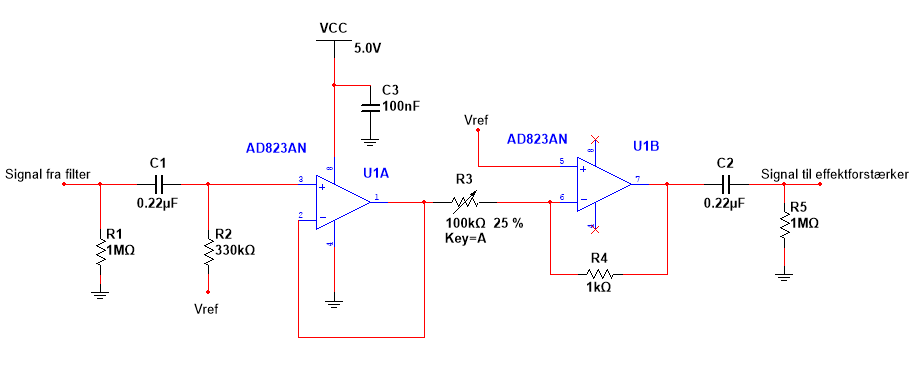
\includegraphics[width=\textwidth]{figure/kreds1}
	\caption{Forstærker kredsløb}
	\label{fig:kreds1}
\end{figure}
Figur \ref{fig:kreds1} viser kredsløbet for vores variabel forstærker. Forstærkerens gain factor varieres fra afstandssensoren R3.

Først regnes støjen fra opamp U1A. Denne støj bliver forstærket op af OpAmp U1B. Herefter ses på bidraget fra R3 alene, som også bliver forstærket op a U1B. Dernæst ser vi på bidraget fra U1B alene. Disse 3 værdier kvardreres, summeres og vi tager roden af dem, for at finde det samlede bidrag før ADC'en. Sidst regnes det samlede støjbidrag, som vi nu kan sammenligne vores simulering og realisering med.

\subsection{Støj fra OpAmp U1A}


VÆRDIER IKKE REDIGERET ENDNU

\begin{align*}
e\tsub{n} &= \SI{43}{\nano\voltnoise}
\\[2.0ex]
B &= \frac{ \SI{10}{\mega\hertz}}{\SI{50}{\volt\per\volt}}
\\[2.0ex]
&= \SI{180}{\kilo\hertz}
\\[2.0ex]
V\tsub{o\_rms} &= \left| A_1\cdot A_2 \cdot e\tsub{n} \right| \cdot \sqrt{B}
\\[2.0ex]
&= \SI{50}{\volt\per\volt} \cdot \SI{15}{\volt\per\volt} \cdot \SI{43}{\nano\voltnoise} \cdot \sqrt{\SI{180}{\kilo\hertz}}
\\[2.0ex]
&= \SI{13.7}{\milli\volt}
\end{align*}


\subsection{Støj fra variabel modstand R3}

VÆRDIER IKKE REDIGERET ENDNU

\begin{align*}
V\tsub{rms\_tæthed} &= \sqrt{4 \cdot k \cdot T \cdot R}
\\[2.0ex]
&= \sqrt{4 \cdot k\cdot \SI{313}{\kelvin} \cdot \SI{10}{\kilo\ohm}}
\\[2.0ex]
&= \SI{18.7}{\nano\voltnoise}
\\[2.0ex]
V\tsub{rms\_forstærket} &= \SI{18.7}{\nano\voltnoise} \cdot 50
\\[2.0ex]
&= \SI{935}{\nano\voltnoise}
\end{align*}

\subsection{Støj fra OpAmp U1B}

VÆRDIER IKKE REDIGERET ENDNU

\begin{align*}
e\tsub{n} &= \SI{43}{\nano\voltnoise}
\\[2.0ex]
B &= \frac{ \SI{10}{\mega\hertz}}{\SI{50}{\volt\per\volt}}
\\[2.0ex]
&= \SI{180}{\kilo\hertz}
\\[2.0ex]
V\tsub{o\_rms} &= \left| A_1\cdot A_2 \cdot e\tsub{n} \right| \cdot \sqrt{B}
\\[2.0ex]
&= \SI{50}{\volt\per\volt} \cdot \SI{15}{\volt\per\volt} \cdot \SI{43}{\nano\voltnoise} \cdot \sqrt{\SI{180}{\kilo\hertz}}
\\[2.0ex]
&= \SI{13.7}{\milli\volt}
\end{align*}

Vi kan nu finde det samlede støjbidrag, før ADC'en:

\begin{align*}
V\tsub{rmstotal} &= \sqrt{\SI{12}{\milli\volt^2} + \SI{12}{\milli\volt^2} + \SI{12}{\milli\volt^2}} = \SI{36}{\milli\volt}
\end{align*}


\subsection{Støj fra ADC'en}





\section{Simulering}

\section{Realisering}

\section{Konklusion}

\end{document}